\documentclass[12pt]{report}

\usepackage[a4paper,pdftex]{geometry}	% Use A4 paper margins
\usepackage[english]{babel}
\usepackage{xcolor} % Required for specifying custom colors
\usepackage{fix-cm} % Allows increasing the font size of specific fonts beyond LaTeX default specifications
\usepackage[hidelinks]{hyperref}
\usepackage{parskip}
\usepackage{color}
\usepackage{picture}
\usepackage{setspace}
\usepackage{amssymb}
\usepackage{mathtools}
\usepackage{graphicx}
\usepackage{floatrow}
\usepackage[labelformat=empty]{caption}


\usepackage{listings}
\usepackage{color}
 
\definecolor{dkgreen}{rgb}{0,0.6,0}
\definecolor{gray}{rgb}{0.5,0.5,0.5}
\definecolor{mauve}{rgb}{0.58,0,0.82}
 
\lstset{ %
  language=Octave,                % the language of the code
  basicstyle=\footnotesize,           % the size of the fonts that are used for the code
  backgroundcolor=\color{white},      % choose the background color. You must add \usepackage{color}
  showspaces=false,               % show spaces adding particular underscores
  showstringspaces=false,         % underline spaces within strings
  showtabs=false,                 % show tabs within strings adding particular underscores
  frame=single,                   % adds a frame around the code
  rulecolor=\color{black},        % if not set, the frame-color may be changed on line-breaks within not-black text (e.g. commens (green here))
  tabsize=2,                      % sets default tabsize to 2 spaces
  captionpos=b,                   % sets the caption-position to bottom
  breaklines=true,                % sets automatic line breaking
  breakatwhitespace=false,        % sets if automatic breaks should only happen at whitespace
  title=,                   % show the filename of files included with \lstinputlisting;
                                  % also try caption instead of title
  keywordstyle=\color{blue},          % keyword style
  commentstyle=\color{dkgreen},       % comment style
  stringstyle=\color{mauve},         % string literal style
  escapeinside={\%*}{*)},            % if you want to add LaTeX within your code
  morekeywords={*,...}               % if you want to add more keywords to the set
}


\setlength{\oddsidemargin}{0mm} % Adjust margins to center the colored title box
\setlength{\evensidemargin}{0mm} % Margins on even pages - only necessary if adding more content to this template

\newcommand{\HRule}[1]{\hfill \rule{0.2\linewidth}{#1}} % Horizontal rule at the bottom of the page, adjust width here

\definecolor{grey}{rgb}{0.9,0.9,0.9} % Color of the box surrounding the title - these values can be changed to give the box a different color	

\begin{document}

\thispagestyle{empty} % Remove page numbering on this page

%----------------------------------------------------------------------------------------
%	TITLE SECTION
%----------------------------------------------------------------------------------------

\colorbox{grey}{
	\parbox[t]{1.0\linewidth}{
		\centering \fontsize{50pt}{80pt}\selectfont % The first argument for fontsize is the font size of the text and the second is the line spacing - you may need to play with these for your particular title
		\vspace*{0.7cm} % Space between the start of the title and the top of the grey box
		
		\hfill Siminov Framework Version 0.9.1-Beta\\
		\hfill Getting Started Guide\par
		
		\vspace*{0.7cm} % Space between the end of the title and the bottom of the grey box
	}
}

%----------------------------------------------------------------------------------------

	\vfill % Space between the title box and author information

%----------------------------------------------------------------------------------------
%	AUTHOR NAME AND INFORMATION SECTION
%----------------------------------------------------------------------------------------

	{\centering \large 
\hfill Siminov Framework\\
\hfill \texttt{http://www.siminov.github.com/android-orm} \\

\HRule{1pt}} % Horizontal line, thickness changed here

%----------------------------------------------------------------------------------------

\clearpage % Whitespace to the end of the page


\noindent
%%%%%%%%%%%%%%%%%%%%%%%%%%%%%%%%%%%%%%%%%%%%%%%%%%%%%%%%%%%%%%%%%%%%%%%%%%%%%%%%%%%%%%%%%%%%%%%%%%%%%%%%%%%%%%%%%%%%%%%%
%set the number of sectioning levels that get number and appear in the contents
\pagenumbering{gobble}
\setcounter{secnumdepth}{3}
\setcounter{tocdepth}{3}


\tableofcontents

%%%%%%%%%%%%%%%%%%%%%%%%%%%%%%%%%%%%%%%%%%%%%%%%%%%%%%%%%%%%%%%%%%%%%%%%%%%%%%%%%%%%%%%%%%%%%%%%%%%%%%%%%%%%%%%%%%%%%%%%

%%%%%%%%%%%%%%%%%%%%%%%%%%%%%%%%%%%%%%%%%%%%%%%%%%%%%%%%%%%%%%%%%%%%%%%%%%%%%%%%%%%%%%%%%%%%%%%%%%%%%%%%%%%%%%%%%%%%%%%%
\newpage
\addcontentsline{toc}{chapter}{Preface}
\begin{flushleft}
	\textbf{\emph{\Large{Preface}}}
\end{flushleft}

\small
Working with both Object-Oriented software and Relational Databases can be cumbersome and time consuming. Development costs are significantly higher due to a paradigm mismatch between how data is represented in objects versus relational databases. Siminov is an Object/Relational Mapping solution for Android environments. The term Object/Relational Mapping refers to the technique of mapping data from an object model representation to a relational data model representation (and visa versa). See \url{http://en.wikipedia.org/wiki/Object-relational_mapping} for a good high-level discussion.


\begin{center}
	\colorbox{grey}{
		\parbox[t]{.8\linewidth}{
			\fontsize{11pt}{11pt}\selectfont % The first argument for fontsize is the font size of the text and the second is the line spacing - you may need to play with these for your particular title
			\vspace*{0.7cm} % Space between the start of the title and the top of the grey box
		
			\hfill \textbf{Note} \\
			\hfill While having a strong background in SQL is not required to use Android-Siminov, having a basic understanding of the concepts can greatly help you understand Siminov more fully and quickly. Probably the single best background is an understanding of data modeling principles. You might want to consider these resources as a good starting point: \url{http://en.wikipedia.org/wiki/Data_modeling}\\
		
			\vspace*{0.7cm} % Space between the end of the title and the bottom of the grey box
		}
}

\end{center}


Siminov not only takes care of the mapping from Java classes to database tables (and from Java data types to SQL data types), but also provides data query and retrieval facilities. It can significantly reduce development time otherwise spent with manual data handling in SQLite. Siminov design goal is to relieve the developer from 99% of common data persistence-related programming tasks by eliminating the need for manual, hand-crafted data processing using SQLite. However, unlike many other persistence solutions, Siminov does not hide the power of SQLite from you and guarantees that your investment in relational technology and knowledge is as valid as always.

Siminov may not be the best solution for data-centric applications that only use stored-procedures to implement the business logic in the database, it is most useful with object-oriented domain models and business logic in the Java-based. However, Siminov can certainly help you to remove or encapsulate vendor-specific SQLite code and will help with the common task of result set translation from a tabular representation to a graph of objects.


\section{Get Involved}

Use Siminov and report any bugs or issues you find. See \url{https://github.com/Siminov/android-orm/issues} for details. Try your hand at fixing some bugs or implementing enhancements. Again, see \url{https://github.com/Siminov/android-orm/issues}. Engage with the community using mailing lists, forums, IRC, or other ways listed at \url{https://github.com/Siminovl}. Help improve or translate this documentation. Contact us on the developer mailing list if you have interest.Spread the word. Let the rest of your organization know about the benefits of Siminov.


\section{Getting Started Guide}

New users may want to first look through the Siminov Getting Started Guide for basic information as well as tutorials. Even seasoned veterans may want to considering perusing the sections pertaining to build artifacts for any changes.

%%%%%%%%%%%%%%%%%%%%%%%%%%%%%%%%%%%%%%%%%%%%%%%%%%%%%%%%%%%%%%%%%%%%%%%%%%%%%%%%%%%%%%%%%%%%%%%%%%%%%%%%%%%%%%%%%%%%%%%%
\newpage
\chapter {\Large{Obtaining Siminov}}



\subsection{Release Bundle Downloads}
The Siminov Framework team provide release bundles hosted at \textbf{Github} File Release System, in ZIP and TGZ formats. Each release bundle contains JARs, documentation, source code, and other goodness.

\par
You can download releases of Siminov Framework, in your chosen format, from the list at \url{http://siminov.github.io/android-orm/index.html}. 

	\begin{enumerate}

		\item \small The lib/required/ directory contains all the JARs Siminov requires. All the jars in this directory must also be included in your project's classpath.

	\end{enumerate}


%%%%%%%%%%%%%%%%%%%%%%%%%%%%%%%%%%%%%%%%%%%%%%%%%%%%%%%%%%%%%%%%%%%%%%%%%%%%%%%%%%%%%%%%%%%%%%%%%%%%%%%%%%%%%%%%%%%%%%%%
\newpage
\chapter {\Large{Setting Up Application}}

\begin{enumerate}

	\item \small Download Siminov jar from \url{http://siminov.github.io/android-orm/builds.html}

	\item \small Add Siminov jar into your application libs folder.

		\par
		\textbf{Example:} Siminov Template Application
		\begin{figure}[htbp]
			\centering
				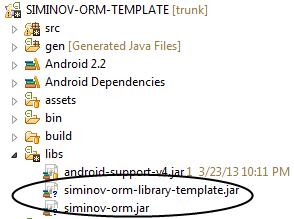
\includegraphics[height=8cm]{Resources/siminov_template_application_add_siminov_jar.png}
		\end{figure}


\end{enumerate}
%%%%%%%%%%%%%%%%%%%%%%%%%%%%%%%%%%%%%%%%%%%%%%%%%%%%%%%%%%%%%%%%%%%%%%%%%%%%%%%%%%%%%%%%%%%%%%%%%%%%%%%%%%%%%%%%%%%%%%%%
\newpage
\chapter {\Large{Building Application}}
Building application based on Siminov Framework is easy, simple. By the help of \textbf{Siminov Template Application} we will explain how we can build application.


\section{Configure ApplicationDescriptor.si.xml}
Application Descriptor is the one who connects application to Siminov Framework. It provide basic information about application, which defines the behaviour of application.

	\lstinputlisting[language=xml]{Resources/siminov_template_application_application_descriptor.txt}



\section{Configure DatabaseDescriptor.si.xml}
Database Descriptor is the one who denes the schema of database.

	\lstinputlisting[language=xml]{Resources/siminov_template_application_database_descriptor.txt}


\section{Configure LibraryDescriptor.si.xml}
Library Descriptor is the one who denes the properties of library.


	\lstinputlisting[language=xml]{Resources/siminov_library_template_library_descriptor.txt}


\section{Configure DatabaseMappingDescriptor.si.xml}
Database Mapping Descriptor is one which does ORM, it maps POJO class to database table.

	\lstinputlisting[language=xml]{Resources/siminov_template_application_database_mapping_descriptor.txt}



\section{Using Annotation}
Liquor pojo class of Siminov template application.

	\lstinputlisting[language=Java]{Resources/siminov_template_application_liquor_pojo_class.txt}


\section{Saving Entity Object}
Saving liquor entity object.

	\lstinputlisting[language=Java]{Resources/siminov_template_application_saving_liquor_object.txt}


\section{Updaing Entity Object}
Updating liquor object.

	\lstinputlisting[language=Java]{Resources/siminov_template_application_updating_liquor_object.txt}


\section{Save Or Update Entity Object}
Save or update liquor object.

	\lstinputlisting[language=Java]{Resources/siminov_template_application_save_or_update_liquor_object.txt}



\section{Deleting Entity Object}
Deleting liquor object.

	\lstinputlisting[language=Java]{Resources/siminov_template_application_deleting_liquor_object.txt}





\end{document}